\chapter{Forord}
Denne rapport er skrevet på 3. semester af gruppe 10, på retningerne IKT og EE ved Aarhus Universitet, Ingeniørhøjskolen.
Vejleder for dette projekt er Søren Hansen. Afleveringsdatoen for denne projektrapport er den 20. december 2016, og bedømmelse er den 18. januar 2017.
Rapporten er udarbejdet på baggrund af den dokumentation, som kan findes i bilaget for projektrapporten.

\section{Læsevejledning}
Rapporten er inddelt i nummererede kapitler. Hvert kapitel indeholder nummererede sektioner med dertil hørende undersektioner. Nedenunder er givet eksempler på disse. \\

\begin{figure}[H]
	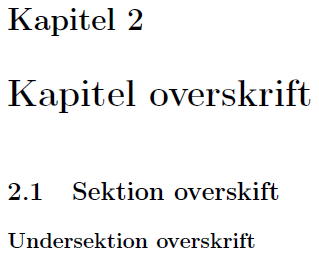
\includegraphics{KapitelStoerrelse.png}
\end{figure}

\noindent
Der vil blive brugt initialer på gruppens medlemmer til angivelse af, hvem rapportens sektioner er skrevet af: \\
\\
Mikkel Busk Espersen (MBE), \\
Jacob Munkholm Hansen(JMH), \\
Ahmad Sabah (AS), \\
Halfdan Vanderbruggen Bjerre(HVB). \\
\\
I de udarbejdede UML- og SysML-diagrammer og beskrivelser af disse vil der blive refereret til p- og s-motorer. Disse dækker over motorerne til styring af 
henholdsvis åbningsmekanismen\footnote{Se ordliste i bilag} og skruen.

\section{Hovedansvarsområder}
Tabel \ref{tab:ansvar} viser fordelingen af hovedansvarsområder for produktet fordelt på gruppemedlemmer. Emnerne er inddelt i primær og sekundær, som informerer om 
medlemmers specialistviden og kernekompetencer indenfor produktudviklingen. Enkelte sekundære felter er tomme, dette betyder at ingen har været sekundær på 
emnet.

\begin{table}[H]
	\centering
	\begin{tabular}{| l | c | c |}
		\hline
		Emne & Primær & Sekundær\\\hline
		Brugergrænseflade (GUI) & AS & HVB\\\hline
		SPI DevKit-PSoC & HVB & JMH\\\hline
		SPI PSoC-PSoC & HVB, JMH & \\\hline
		PSoC software sensor & JMH & MBE\\\hline
		PSoC software sensor & JMH & MBE\\\hline
		Bipolære motorer & MBE & JMH\\\hline
		Unipolære motorer & MBE & JMH\\\hline
		DC motor & MBE & \\\hline
		Konstruktion og mekanik & AS & HVB\\\hline
	\end{tabular}
	\caption{Fordeling af hovedansvarsområder}
	\label{tab:ansvar}
\end{table}